\subsection{Вырожденные звёзды}
\term{Вырожденные звезды}~--- звезды, в которых силам гравитации противостоят силы давление вырожденного газа. К таким относятся \imp{белые карлики} и \imp{нейтронные звезды}. 

\begin{figure}[!h]
	\centering
	\begin{minipage}[c]{0.49\tw}
 		\begin{tikzpicture}
 			\begin{axis}[
 							height	=	4.5cm,
 							width	=	\tw,
 							xlabel	=	{Фаза}, 
 							ylabel	=	{Блеск $m$, $~^m$}, 
 							ymax	=	.7,
 							ymin	=	-.1,
 							y dir	=	reverse,
 							xmax	=	1,
 							xmin	=	.0
 						]
				\addplot[smooth] table[x=t, y=m]{data/light-curve-B-Lyr.txt};
 			\end{axis}
 		\end{tikzpicture}
 	\end{minipage}
 	\hfill
 	\begin{minipage}[c]{0.49\tw}
 		\centering
 		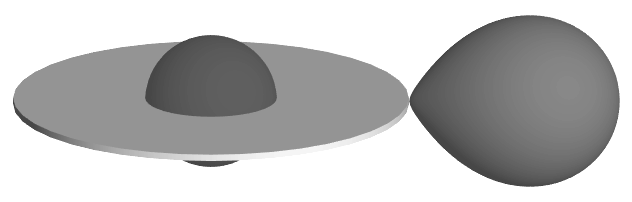
\includegraphics[width = .9\tw]{b-lyr}	
 	\end{minipage}
 	\caption{Кривая блеска переменной типа $\beta$\,Lyr}
 	\label{pic:b-lyr}
 	\vspace{-.8pc}
\end{figure}
\term{Белые карлики}~--- проэволюционировавшие звёзды лишённые собственных источников термоядерной энергии и светящие за счёт остывания. Масса белого карлика находится в диапазоне от $0.6M_{\odot}$ до $1.44 M_{\odot}$. Верхняя границы массы белого карлика называется пределом Чандрасекара, звезда с массой больше данного предела не может существовать как белый карлик. Радиус белых карликов примерно в $10^2$ раз меньше солнечного, т.е. можно считать, что $R_\text{БК} \simeq R_\oplus$. Плотность белых карликов лежит в диапазоне $10^7$\,--\,$10^{10}$~$\text{кг}/\text{м}^3$.

\term{Нейтронная звезда}~--- сверхплотная звезда, образующаяся в результате взрыва Сверхновой. Вещество нейтронной звезды состоит в основном из нейтронов. Масса нейтронной звезды лежит в пределах от $0.1M_{\odot}$ до $2$\,--\,$2.8M_{\odot}$ (предел Оппенгеймера-Волкова). Размер данной звезды составляет лишь $10$\,--\,$20$~км, а плотность составляет $10^{16}$\,--\,$10^{18}$ $\text{кг}/\text{м}^3$.  Дальнейшему гравитационному сжатию нейтронной звезды препятствует давление ядерной материи, возникающее за счёт взаимодействия нейтронов. Так как нейтронные звёзды образуются в результате  коллапса массивных звёзд, то из-за сохранения момента импульса скорость их вращения может достигать $10^5$~км/с. При наличии сильного магнитного поля и быстром вращении нейтронная звзеда может наблюдаться с Земли как \term{пульсар}.